%
% This document is licensed under the
%
%   Creative Commons Attribution-Noncommercial-Share Alike
%
% license. Please see LICENSE file for details.
%

\documentclass{InsightArticle}

\usepackage[dvipdfmx]{graphicx}
\usepackage{url}
\usepackage{textcomp}

\usepackage[dvipdfmx,
bookmarks,
bookmarksopen,
backref,
colorlinks,linkcolor={blue},citecolor={blue},urlcolor={blue},
]{hyperref}


\title{Unwarping Echo Planar Images Using CMTK\footnote{This document is licensed under
    the Creative Commons Attribution License Version 3.0.}}

\release{1.0}

\author{Torsten Rohlfing}
\authoraddress{Neuroscience Program, SRI International, Menlo Park, CA}

\begin{document}

\maketitle

\ifhtml
\chapter*{Front Matter\label{front}}
\fi


\begin{abstract}
\noindent This document describes the workflow for unwarping echo planar MR
images (EPI), in particular diffusion-weighted images, using an acquisition
method with reversed phase encoding and the tools of the Computational
Morphometry Toolkit (CMTK). This technique requires an additional acquisition
(additional $b=0$ image for diffusion imaging) with reversed phase encoding
direction, but no field map. Simple 6-direction diffusion data are provided
with this article for demonstration.
\end{abstract}

\tableofcontents

\clearpage
\section{Introduction}

Echo-planar images are essential for the acquisition of diffusion weighted as
well as functional (i.e., BOLD) MR images. Unfortunately, these images are
subject to significant spatial distortions to due susceptibility changes at,
for example, air-tissue boundaries.

The most common technique to correct these distortions is via the acquisition
of a field map, from which the distortion field can be computed. This has
several disadvantages, such as the need to acquire the field maps, and the
need to compute unwrapped phase maps. Also, the resulting distortion
correction is not necessarily of good quality.

Holland {\em et al.\/}~\cite{HollKupeDale:2010} have recently introduced a
field map-free undistortion method, which makes use of the fact that the
distortion behaves ``symmetrically'' when the phase encoding direction of the
acquisition is reversed.

Thus, from a pair of images acquired with opposing phase encoding direction,
one can compute a symmetric deformation field pair that undistorts both input
images. If this is done for a pair of opposing-phase-encode $b=0$ images in
diffusion images, and the actual diffusion-weighted images are acquired
analogous to one of the two $b=0$ images, then the entire set of diffusion
images can be unwarped using the deformation field computed for the
appropriate $b=0$ image.

We describe herein the tools of the Computational Morphometry Toolkit (CMTK),
which implement the numerical computational part of this unwarping
strategy. Demonstration data are provided with this article to test the
described tools and workflows.

\subsection{CMTK}

The Computational Morphometry Toolkit (CMTK) is {\bf free software}, and
that's as in both free beer and free speech. CMTK is available both in source
code, licensed under the GPLv3, and as pre-compiled binary distributions from
\url{http://nitrc.org/projects/cmtk/}. If you are using NeuroDebian, you can
also install CMTK directly.

We shall assume that CMTK has been installed such that its tools can be run as
\begin{verbatim}
cmtk <tool> <arg1> <arg2> ...
\end{verbatim}

{\bf To perform the processing stages described in this article, you will need
CMTK release 2.2.4 or later.} Versions prior to 2.2.0 do not support EPI
unwarping, and versions 2.2.0 through 2.2.3 contain a bug that prevented
proper initialization of the deformation field in some cases.

\section{Step-by-Step}

\subsection{Imaging}

On your MR scanner of choice, you will need to implement an acquisition like
the one described in Ref.~\cite{HollKupeDale:2010}. In short, before the $b=0$
image of your favourite DWI acquisition sequence, you need to acquire an
additional $b=0$ image with phase-encoding direction reversed, thus resulting
in an image that is flipped in the phase-encoding direction and also distorted
by the ``opposite'' distortion field. 

{\bf Note that CMTK will not help you set up the acquisition - this is outside
the scope of the toolkit and also outside the scope of this manual.}

\begin{figure}[tbp]
\begin{center}
\begin{tabular}{cc}
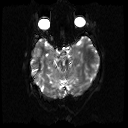
\includegraphics[width=.475\linewidth]{eps/b0_bwd} &
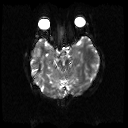
\includegraphics[width=.475\linewidth]{eps/b0_fwd} \\
(a) \texttt{b0\_bwd.nii.gz} & (b)  \texttt{b0\_fwd.nii.gz}\\
\\
\end{tabular}
\begin{tabular}{ccc}
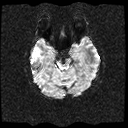
\includegraphics[width=.31\linewidth]{eps/b1} &
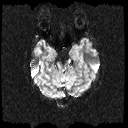
\includegraphics[width=.31\linewidth]{eps/b2} &
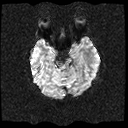
\includegraphics[width=.31\linewidth]{eps/b3} \\
(c) \texttt{b1.nii.gz} & (d) \texttt{b2.nii.gz} & (e) \texttt{b3.nii.gz} \\
\\
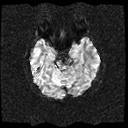
\includegraphics[width=.31\linewidth]{eps/b4} &
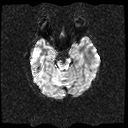
\includegraphics[width=.31\linewidth]{eps/b5} &
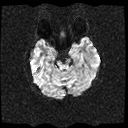
\includegraphics[width=.31\linewidth]{eps/b6} \\
(f) \texttt{b4.nii.gz} & (g) \texttt{b5.nii.gz} & (h) \texttt{b6.nii.gz} \\
\end{tabular}
\end{center}
\caption{Demonstration data provided with this paper (file names given in
  parentheses). (a) Axial slice from $b=0$ image acquired with reversed phase-encoding
  direction. (b) Same slice from $b=0$ image acquired with standard
  phase-encoding direction. (c) through (h) Same slice from six different
  diffusion-weighted images acquired with standard phase-encoding direction.}
\label{fig:B0FwBw}
\end{figure}

\subsection{DICOM Image Stacking}

Assume that the DICOM files containing the EPI data are stored in the
``\texttt{dicom/}'' directory. These are stacked into 3D images in
NIFTI-format using the following CMTK command:
\begin{verbatim}
cmtk dcm2image -vx -O dwi/image%n.nii dicom/
\end{verbatim}

This will result in a series of continuously numbered images in NIFTI format,
all stored in the <tt>dwi/</tt> directory.

Let us assume that we are using a 6-gradient-direction DWI setup with a single
reverse phase-encoded $b=0$ image acquired first, followed by the standard
$b=0$ image, followed by six diffusion images with different gradient
directions. In this case, we should find the following files:
\begin{description}
\item[\tt image1.nii] -- reverse phase-encoded $b=0$ image
\item[\tt image2.nii] -- standard phase-encoded $b=0$ image
\item[\tt image3.nii] -- 1st diffusion image
\item[\tt image4.nii] -- 2nd diffusion image
\item[\tt image5.nii] -- 3rd diffusion image
\item[\tt image6.nii] -- 4th diffusion image
\item[\tt image7.nii] -- 5th diffusion image
\item[\tt image8.nii] -- 6th diffusion image
\end{description}

\subsection{Unwarping EPI}

First, we compute the deformations to unwarp the two opposite-direction phase
encoded $b=0$ images. We also write out the Jacobian determinant map of the
forward-encoded image, which we will need to correct for signal pile up:
\begin{verbatim}
cmtk epiunwarp --write-jacobian-fwd epiunwarp/jacobian_fwd.nii \
  inputs/b0_bwd.nii.gz inputs/b0_fwd.nii.gz \
  epiunwarp/b0_bwd.nii epiunwarp/b0_fwd.nii epiunwarp/dfield.nrrd
\end{verbatim}
Second, apply the computed deformation to the first diffusion-weighted image
(analogous to the remaining diffusion images) to create an unwarped
reformatted image:
\begin{verbatim}
cmtk reformatx --floating inputs/b1.nii --linear -o epiunwarp/b1.nii \
  epiunwarp/b0_fwd.nii epiunwarp/dfield.nrrd
\end{verbatim}
Third, compute the pixel-wise multiplication of the unwarped diffusion image
with the Jacobian of the deformation:
\begin{verbatim}
cmtk imagemath --in epiunwarp/b1.nii epiunwarp/jacobian_fwd.nii --mul \
  --out epiunwarp/b1.nii
\end{verbatim}
The result is the final, distortion-corrected image.

\subsection{Unwarping EPI with Eddy-Current Correction}

\begin{verbatim}
cmtk correct_dwi_distortion unwarp_eddy \
  inputs/b0_bwd.nii.gz inputs/b0_fwd.nii.gz inputs/b?.nii.gz
\end{verbatim}

\subsection{Unwarping EPI with Eddy Current and Subject Motion Correction}

\begin{verbatim}
cmtk correct_dwi_distortion_and_motion unwarp_eddy_motion \
  inputs/b0_bwd.nii.gz inputs/b0_fwd.nii.gz inputs/b?.nii.gz
\end{verbatim}

\section*{Acknowledgments}

\bibliographystyle{UnwarpEchoPlanar}
\bibliography{UnwarpEchoPlanar}

\end{document}

